\documentclass[11pt]{nodycon2021}
\usepackage{epsfig,amsmath,amsfonts}

%%
\let\OLDthebibliography\thebibliography
\renewcommand\thebibliography[1]{
  \OLDthebibliography{#1}
  \setlength{\parskip}{0pt}
  \setlength{\itemsep}{0pt plus 0.3ex}
}
\usepackage[official]{eurosym}
%%%

\title{Solving Non-smooth Dynamic Problems using \\ the 
Alternating Direction Method of Multipliers }

\author{\textbf{Alessandro Tasora}$^\ast$, Dario Mangoni$^\ast$ and Simone Benatti$^{\ast\ast}$}

\address{$^\ast$Department of Engineering and Architecture, University of Parma, ITALY}

\abstract{We propose to use the Alternating Direction Method of Multipliers (ADMM) for solving the variational inequality that arises in non-smooth contact problems in multibody simulations. The ADMM method is based on simple computational primitives, it scales well with the problem size, it can handle problems that mix finite elements and rigid bodies, it offers superior convergence properties.}

\begin{document}
%%%%%%%%%%%%%%%%%%%%%%%%%%%%%%%%%%%%%%%%%%%%%%%%%%%%%%%%%%%%
\section{Introduction}

Non-smooth dynamical problems, such as those involving contact and friction, can be solved by means of special time stepping methods that offer superior robustness and stability at the cost of solving a variational inequality per each time step.
% \cite{acary2008numerical}. 
Under mild assumptions such variational inequality can be stated as a convex cone complementarity problem, that can be also cast as an optimization problem, namely a quadratic program with convex constraints \cite{anitescuTasora2008}. During the last years, different numerical methods have been proposed to solve such problem: fixed point iterations such as projected Jacobi, first-order spectral methods such as SPG, Interior Point (IP) methods and others. Recently there has been a revival of Alternating Direction Method of Multipliers (ADMM) and similar operator-splitting methods for solving this class of problems \cite{Goldstein2014}. %  [2014 Alternating Direction Optimization Methods]. 
Even if the theoretical convergence of such methods is worse than the one of IP methods, recent developments showed that in practical scenarios they offer superior speed, scalability and robustness 
\cite{Cannon2019}. % [COSMO  conic operator splitting method for large convex problems].
In 
\cite{Stellato2020} % [OSQP: an operator splitting solver for quadratic programs].
a specialized ADMM method for quadratic problems with conic constraints has been presented: on the top of this method we develop a solver that can exploit the nature of non-smooth dynamical problems. In our embodiment, unknowns are primal variables (velocity measures) and dual variables (impulses in contact points and joints), cone constraints stem from the Coulomb friction law, and the system matrix includes terms from the mass matrices and from the tangent stiffness/damping matrices (hence it is sparse, but not necessarily diagonal).


\begin{figure}[h!]
\centering
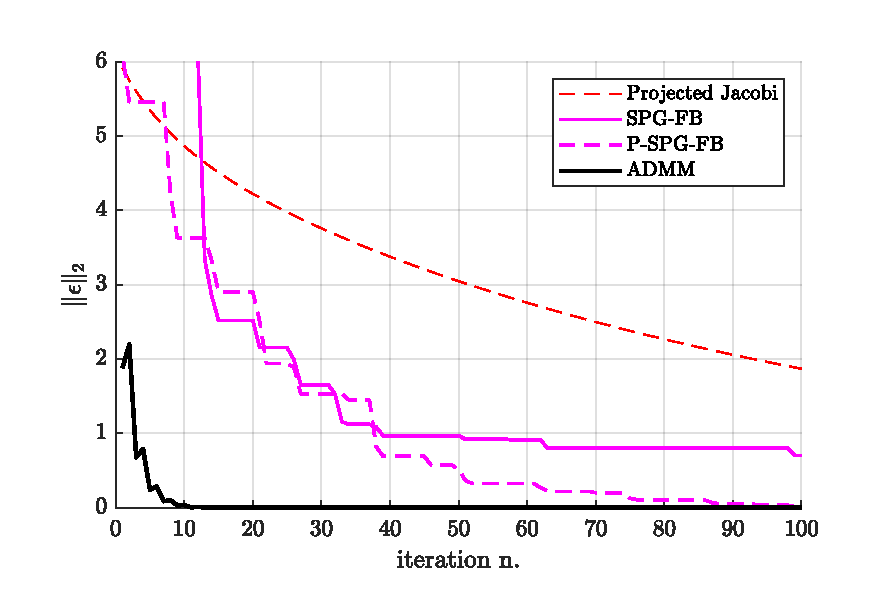
\includegraphics[width=0.50\textwidth]{t8_convergence.pdf}
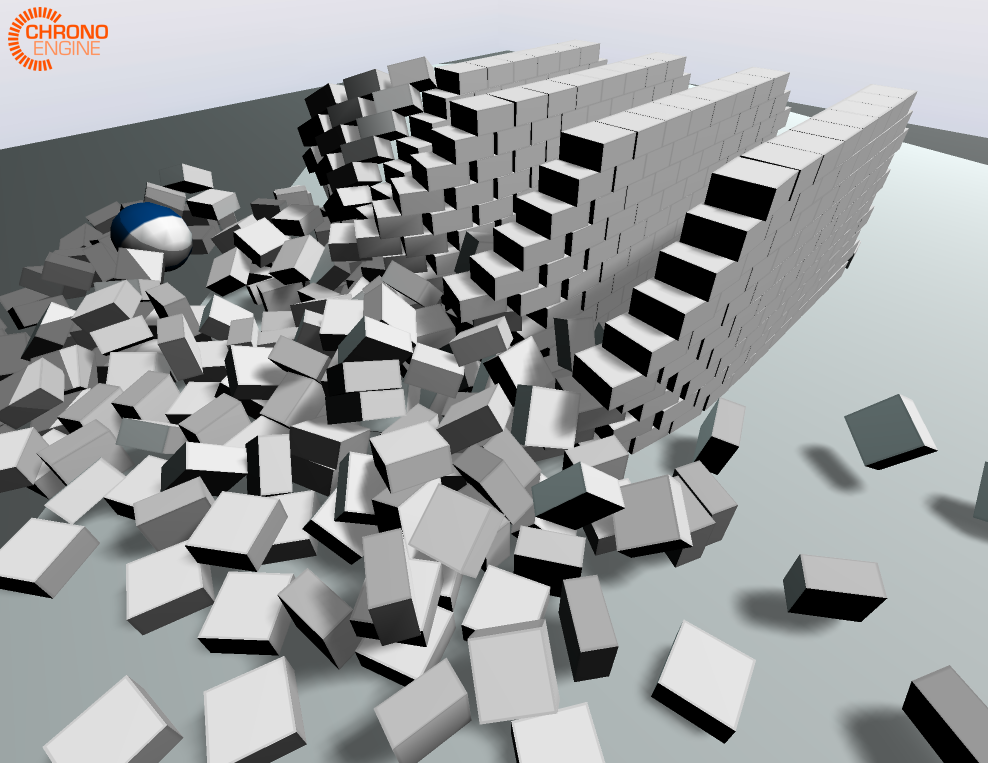
\includegraphics[width=0.35\textwidth, trim=0cm -3cm 0 3cm]{t8_snapshot.png}
\caption{Convergence of the ADMMM method within one time step of the wrecking ball benchmark (600 bricks in four walls): residual in frictional constraint   violation compared to fixed point Jacobi iterations and to first-order SPG methods.}
\end{figure}




\section{Results and discussion}
 
Our ADMM method requires few computational primitives: basically a projection of dual variables on conic sets, a backward solve of a linear system, and a forward solve. The latter is a computational bottleneck, but it can be performed only once per run, as the matrix does not change often during the iterations. 
A good estimation of the ADMM step size proved to be fundamental in achieving good convergence: using some heuristics we obtained an efficient auto-tuning algorithm. 
We noted that ADMM can be successfully applied to problems that exhibit temporal coherence because, unlike IP methods, it supports warm-starting.





\bibliographystyle{svproc}
\bibliography{../../bibliography/refsMBS,../../bibliography/refsOPT}


 \end{document} 